\documentclass[a4paper, 12pt]{article}
\usepackage[a4paper,top=1.5cm, bottom=1.5cm, left=1cm, right=1cm]{geometry}
\usepackage{cmap}
\usepackage{mathtext}
\usepackage[T2A]{fontenc}
\usepackage[utf8]{inputenc}
\usepackage[english,russian]{babel}
\usepackage{multirow}
\usepackage{graphicx}
\usepackage{wrapfig}
\usepackage{tabularx}
\usepackage{float}
\usepackage{wrapfig}
\usepackage{longtable}
\usepackage{booktabs}
\usepackage{hyperref}
\hypersetup{colorlinks=true,urlcolor=blue}
\usepackage[rgb]{xcolor}
\usepackage{amsmath,amsfonts,amssymb,amsthm,mathtools}
\usepackage{icomma}
\usepackage{euscript}
\usepackage{mathrsfs}
\usepackage{enumerate}
\usepackage{caption}
\mathtoolsset{showonlyrefs=true}
\usepackage{subcaption}
\usepackage[europeanresistors, americaninductors]{circuitikz}
\DeclareMathOperator{\sgn}{\mathop{sgn}}
\newcommand*{\hm}[1]{#1\nobreak\discretionary{}
	{\hbox{$\mathsurround=0pt #1$}}{}}

\begin{document}

\newgeometry{left=2cm, right=2cm, top=2cm, bottom=1cm,
             bindingoffset=0cm}

\begin{titlepage}
    \begin{center}
        \vspace*{5cm}
        \Huge МФТИ
        \vspace*{2cm}\\
        \LARGE \textbf{Лабораторная работа}
        \\\vspace*{0.25cm}

        \noindent\rule{\textwidth}{1pt}
        \vspace*{-0.25cm}

        \huge \textbf{Петля Гистерезиса(динамический метод)}
        \noindent\rule{\textwidth}{1pt}

        \vfill

        \begin{flushright}
            \begin{minipage}{.4\textwidth}
            \Large Выполнил: \\ Солодилов Михаил \\ (Б01-306)
            \end{minipage}
        \end{flushright}

        \vfill

        \normalsize Долгопрудный \\2024
    \end{center}
\end{titlepage}

\restoregeometry

\begin{center}
	\section*{Введение}
\end{center}

\begin{flushleft}
  \textbf{Цель работы:} изучение петель гистерезиса раличных ферромагнитных материалов в переменных токах.

\end{flushleft}

\begin{flushleft}
  \textbf{В работе используются:} автотрансформатор, понижающий трансформатор, интегрирующая цепочка, амперметр, вольтметр, электронный осциллограф, делитель напряжения, тороидальные образцы с двумя обмотками (с сердечниками из феррита, пермаллоя и кремнистого железа).

\end{flushleft}

\section*{Теоретическая справка}

Магнитная индукция $B$ и напряжённость поля $H$ в ферромагнитном материале неоднозначно связаны между собой: индукция зависит не только от напряжённости, но и от предыстории образца. Связь между $B$ и $H$ типичного ферромагнетика иллюстрирует рисунок \Ref{Theor}.

\begin{figure}[h]
	\centering
	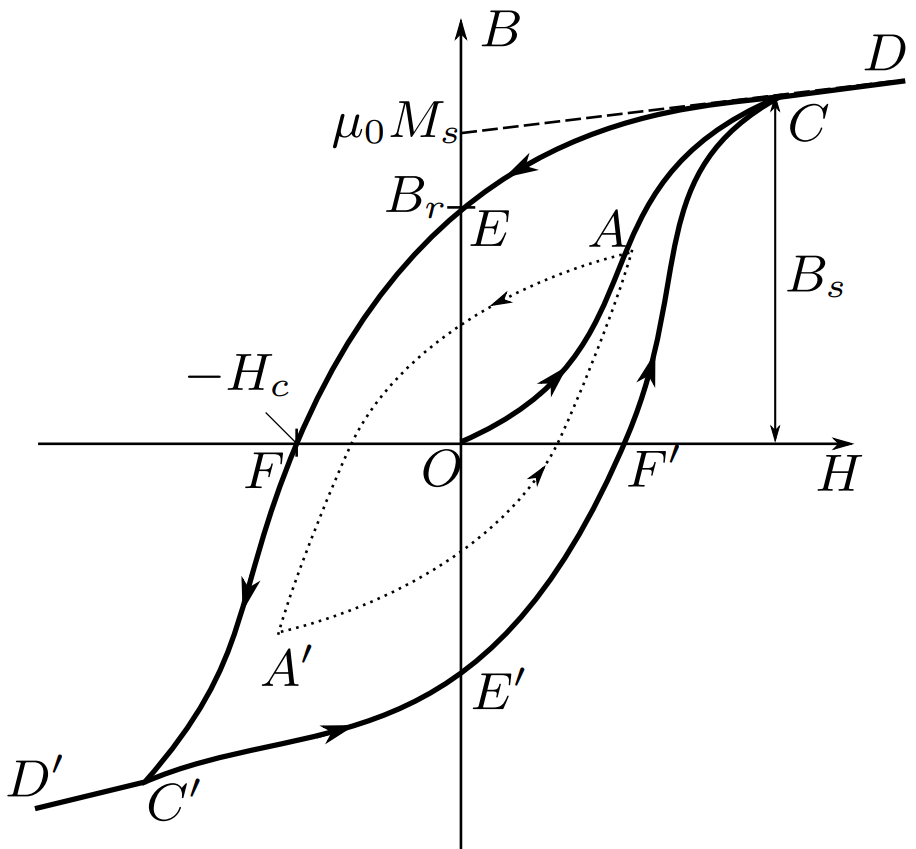
\includegraphics[scale=0.45]{Theor}
	\caption{Петля гистерезиса ферромагнетика} \label{Theor}
\end{figure}

Если к ферромагнитному образцу прикладывать переменное внешнее магнитное поле, то его состояние на плоскости $H-B$ будет изменяться по замкнутой кривой -- \textit{петле гистерезиса}. Резмер петли определяется максимальным значением напряжённости $H$ в цикле (например, петля $AA'$, обозначенная пунктиром на рисунке \Ref{Theor}). Если амплитуда напряжённости достаточно велика, то образец будет периодически достигать \textit{насыщения}, что на рисунке соответствует кривой $CERC'E'F'C$ (\textit{предельная петля гистерезиса}). Пересечение предельной петли с вертикальной осью соответствует остаточной индукции $B_r$, пересечение с горизонтальной осью -- коэрцитивному полю $H_c$. Крайние точки петель, соответствующие амплитудным значениям $H$ (например, точка $A$ на рисунке \Ref{Theor}), лежат на \textit{начальной кривой намагничивания} ($OAC$).

\textbf{Измерение магнитной индукции.} Магнитную индукцию $B$ удобно определять с помощью ЭДС, возникающей при измерении магнитного потока $\Phi$ в катушке, намотанной на образец. Пусть катушка с $N$ витками плотно охватывает образец сечением $S$, и индукция $B$ в образце однородна. Тогда\[\left|B\right|=\frac{1}{SN}\int\varepsilon\text{d}t.\]Таким образом, для определения $B$ нужно проинтегрировать сигнал, наведённый меняющимся магнитным полем в измерительной катушке, намотанной на образец.

Для интегрирования в работе используется \textit{интегрирующая} $RC$-цепочка. Входное напряжение от источника $U_{\text{вх}}(t)$ подаётся на последовательно соединённые резистор $R_{\text{и}}$ и конденсатор $C_{\text{и}}$. Выходное напряжение $U_{\text{вых}}(t)$ снимается с конденсатора. Предположим, что (1) сопротивление источника мало по сравнению с $R_{\text{и}}$; (2) выходное сопротивление (сопротивление на входе осциллографа), напротив, велико: $R_{\text{вых}}\gg R_{\text{и}}$; и, наконец, (3) сопротивление $R_{\text{и}}$ достаточно велико, так что почти всё падение напряжения приходится на него, а $U_{\text{вых}}\ll U_{\text{вх}}$. В таком случае ток цепи равен $I=\frac{U_{\text{вх}}-U_{\text{вых}}}{R_{\text{и}}}\approx\frac{U_{\text{вх}}}{R_{\text{и}}}$, и входное и выходное сопротивление связаны соотношением\[U_{\text{вых}}\frac{q}{C_{\text{и}}}=\frac{1}{C_{\text{и}}}\int_0^tI\text{d}t\approx\frac{1}{\tau_{\text{и}}}\int_0^tU_{\text{вх}}\text{d}t,\]где $\tau_{\text{и}}=R_{\text{и}}C_{\text{и}}$ -- постоянная времени $RC$-цепочки. Для индукции поля получаем\[\left|B\right|=\frac{1}{SN}\int U_{\text{вх}}\text{d}t=\frac{\tau_{\text{и}}}{SN}U_{\text{вх}}.\]

\section*{Экспериментальная установка}

Схема установки приведена на рисунке \Ref{Device}. Напряжение сети (220 Вт, 50 Гц) с помощью регулировочного автотрансформатора Ат через разделительный понижающий трансформатор Тр подаётся на намагничивающую обмотку $N_0$ исследуемого образца.

\begin{figure}[h]
	\centering
	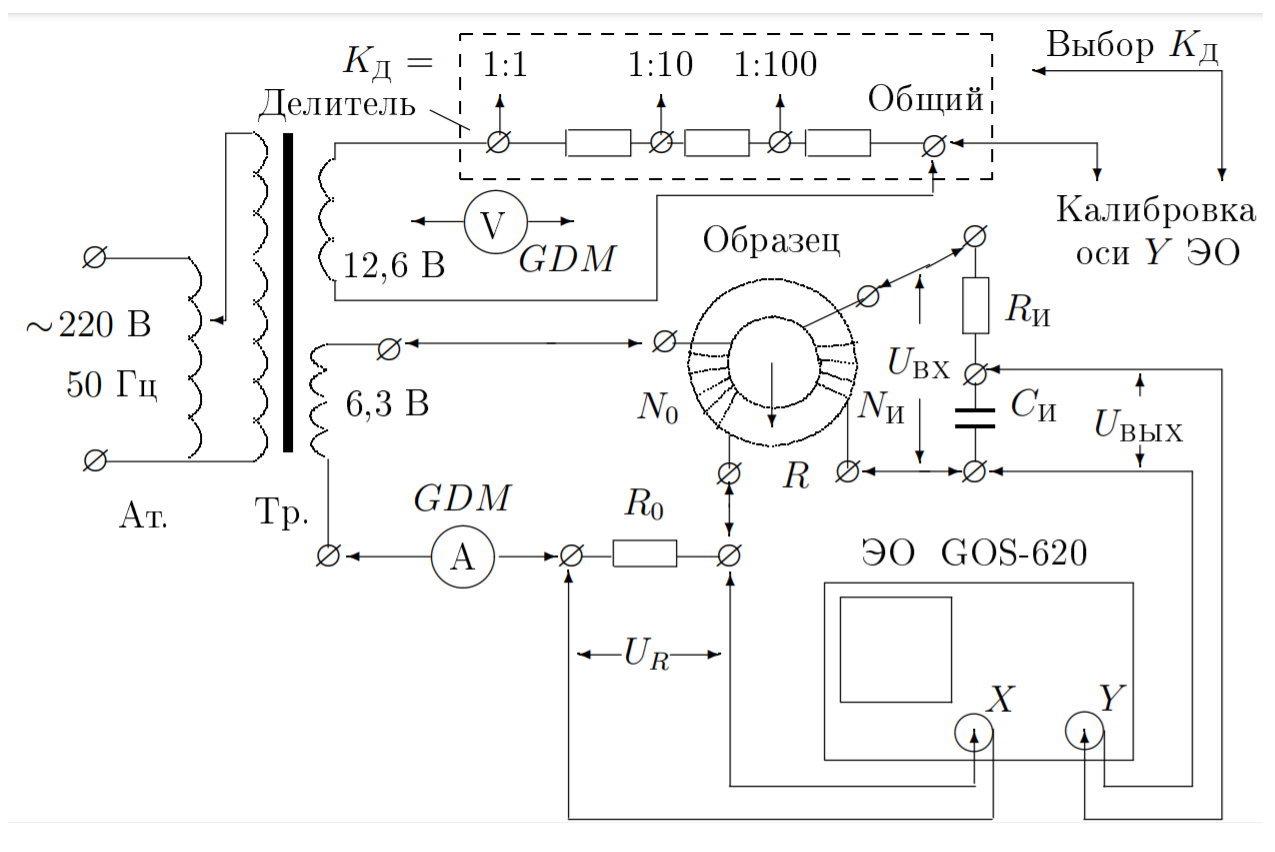
\includegraphics[scale=0.35]{Device}
	\caption{Схема установки для исследования намагничивания образцов} \label{Device}
\end{figure}

Действующее значение переменного тока в обмотке $N_0$ измеряется амперметром $A$ (мультиметром GDM). Последовательно с амперметром включено сопротивление $R_0$, напряжение с которого подаётся на вход $X$ электронного осциллографа (ЭО). Это напряжение пропорционально току в обмотке $N_0$, а следовательно и напряжённости $H$ магнитного поля в образце.

Для измерения магнитной индукции $B$ с измерительной обмотки $N_{\text{и}}$ на вход интегрирующей $RC$-цепочки подаётся напряжение $U_{\text{и}}$ ($U_{\text{вх}}$), пропорциональное производной $\dot{B}$, а с выхода снимается напряжение $U_C$ ($U_{\text{вых}}$), пропорциональное величине $B$, и подаётся на вход $Y$ осциллографа.

Замкнутая кривая, возникающая на экране, воспроизводит в некотором масштабе (различном для осей $X$ и $Y$) петлю гистерезиса. Чтобы придать этой кривой количественный смысл, необходимо установить масштабы изображения, т.е. провести калибровку каналов $X$ и $Y$ ЭО. Для этого, во-первых, надо узнать, каким напряжениям (или токам) соответствуют амплитуды сигналов, видимых на экране, и во-вторых, -- каким значениям $B$ и $H$ соответствуют эти напряжения (или токи).

\textbf{Измерения напряжения с помощью осциллографа.} Исследуемый сигнал подаётся на вход $X$: длина $2x$ горизонтальной черты, наблюдаемой на экране, характризует удвоенную амплитуду сигнала.

Если известна чувствительность усилителя $K_X$ в вольтах на деление шкалы экрана, то удвоенная амплитуда напряжения определяется произведением\[2U_{X,0}=2x\cdot K_X.\]Напряжение, подаваемое на ось $Y$, измеряется аналогично.

Калибровку осей осциллографа ($K_X$ и $K_Y$) можно использовать для построения кривой гистерезиса в координатах $B$ и $H$: зная величину сопротивления $R_0$, с которого снимается сигнал, можно определить чувствительность канала по току $K_{XI}=\frac{K_X}{R_0}\ \left[\frac{\text{А}}{\text{дел}}\right]$ и затем определить цену деления шкалы в $\frac{\text{А}}{\text{м}}$.

Зная чувствительность $K_Y$, можно рассчитать цену деления вертикальной шкалы ЭО в теслах.

Наличие в схеме амперметра и вольтметра позволяет провести \textit{независимую калибровку} усилителей ЭО, т.е. проверить значения коэффициентов $K_X$ и $K_Y$ (ручки регулировки усиления ЭО могут быть сбиты).

\textbf{Проверка калибровки горизонтальной оси ЭО с помощью амперметра} проводится при закороченной обмотке $N_0$. Эта обмотка с помещённым в неё ферромагнитным образцом являеся нелинейным элементом, так что ток в ней не имеет синусоидальной формы, и это не позволяет связать амплитуду тока с показаниями амперметра.

При закороченной обмотке $N_0$ амперметр $A$ измеряет эффективное значение синусоидального тока $I_{\text{эф}}$, текущего через известное сопротивление $R_0$. Сигнал с этого сопротивления подаётся на вход $X$ ЭО. Измерив $2x$ -- длину горизонтальной прямой на экране, можно рассчитать $m_X$ -- чувствительность канала $X$:\[m_X=\frac{2\sqrt2R_0I_{\text{эф}}}{2x}\quad\left[\frac{\text{В}}{\text{дел}}\right].\]

\textbf{Проверка калибровки вертикальной оси ЭО с помощью вольтметра.} Сигнал с обмотки 12,6 В понижающего трансформатора (\Ref{Device}) подаётся на делитель напряжения. Часть этого напряжения снимается с делителя с коэффициентом деления $K_{\text{д}}$ ($\frac{1}{10}$ или $\frac{1}{100}$) и подаётся на вход $Y$ ЭО (вместо напряжения $U_C$). Мультиметр $V$ измеряет напряжение $U_{\text{эф}}$ на этих же клеммах делителя. Измерив $2y$ -- длину вертикальной прямой на экране, можно рассчитать чувствительность канала $Y$:\[m_Y=\frac{2\sqrt2R_0U_{\text{эф}}}{2x}\quad\left[\frac{\text{В}}{\text{дел}}\right].\]

При этом тороид должен быть отключен, так как несинусоидальный ток нагрузки в первичной обмотке тороида приводит к искажению формы кривой напряжения и на обмотке трансформатора, питающей делитель.

\textbf{Постоянную времени RC-цепочки} можно определить экспериментально. С обмотки 6,3 В на вход интегрирующей цепочки подаётся синусоидальное напряжения $U_{\text{вх}}$. На вход $Y$ осциллографа поочерёдно подаются сигналы со входа ($U_{\text{вх}}$) и выхода ($U_{\text{вых}}$) $RC$-цепочки. Измерив амплитуды этих сигналов с помощью осциллографа, можно рассчитать постоянную времени $\tau=RC$. Тогда\[RC=\frac{U_{\text{вх}}}{\Omega U_{\text{вых}}}.\]

\section*{Ход работы}

\subsection*{I. Петля гистерезиса на экране ЭО}

Соберём схему согласно \Ref{Device} и подготовим приборы к работе. Подберём ток питания в намагничивающей обмотке с помощью реостата и коэффициенты усиления ЭО так, чтобы предельная петля гистерезиса занимала большую часть экрана. Получив предельную петлю, уменьшим ток до исчезновения на ней "усов"  \text{--} почти горизонтальных участков по краям. Отцентруем вертикальный и горизонтальный лучи.

Для каждого образца сделаем фотографию предельной петли так, чтобы по ней можно было с хорошей точностью восстановить форму последней. Сфотографируем кривую при ещё двух различных значениях тока при его уменьшении, и полученные оттуда координаты концов частных петель используем для проведения кривой. Эта кривая будет проходить в непосредственной близости от начальной кривой намагничивания. Кривая намагничивания и предельная петля для каждого из образцов показаны на рисунках \Ref{Loop_1}, \Ref{Loop_2} и \Ref{Loop_3}. Кривые проведены с помощью кубических сплайнов.

Рассчитаем цену деления ЭО для петли в $\frac{\text{А}}{\text{м}}$ для оси $X$ по формуле\[H=\frac{N_0K_X}{2\pi RR_0}\]и в $\text{Тл}$ для оси $Y$ \[B=\frac{R_{\text{и}}C_{\text{и}}K_Y}{SN_{\text{и}}}.\]Измерим по предельной петле двойные амплитуды для коэрцитивной силы $\left[2x\left(c\right)\right]$ и индукции насыщения $\left[2y\left(s\right)\right]$. Все измеренные и рассчитанные значения, равно как и параметры образца ($N_0$, $N_{\text{и}}$, $S$ и $2\pi R$), значения коэффициентов усиления $K_X$ и $K_Y$ и ток $I_{\text{эф}}$ в намагничивающей обмотке для каждого образца занесём в сводную талицу \Ref{Table_1}. Занесём туда также вычисленную из наклона кривых намагничивания дифференциальную магнитную проницаемость $\mu_{\text{диф}}$ вблизи нуля и справочные величины для образцов.

Источником погрешностей в финальных ответах служат погрешности чувствительности каналов осциллографа и погрешности определения размеров по экранной сетке осциллографа. В погрешность магнитной проницаемости вносит вклад также неточность определения её по угловому коэффициенту касательной к графику. Опустим вычисление погрешностей ввиду его громоздкости, и приведём их непосредственно в таблице для последних трёх строк.

\begin{table}[h]
	\centering
	\caption{Параметры образцов из (A) пермаллоя, (B) феррита и (C) кремнистого железа} \label{Table_1}
	\begin{tabular}{|c|c|c|c|}
		\hline
		 & A & B & C \\ \hline
		$N_0$ & 35 & 40 & 40  \\ \hline
		$N_{\text{и}}$ & 220 & 400 & 400 \\ \hline
		$S,\ \text{см}^2$ & 3,8 & 3,0 & 1,2 \\ \hline
		$2\pi R$, см & 24 & 25 & 10 \\ \hline
		$I_{\text{эф}}$, А & 0,158 & 0,119 & 0,455 \\ \hline
		$K_X,\ \frac{\text{мВ}}{\text{дел}}$ & 20,0 & 20,0 & 50,0 \\ \hline
		$K_Y,\ \frac{\text{мВ}}{\text{дел}}$ & 100,0 & 10,0 & 50,0 \\ \hline
		$H,\ \frac{\text{А}}{\text{м}}$ & 9,72 & 10,67 & 66,7 \\ \hline
		$B$, Тл & 0,478 & 0,033 & 0,417 \\ \hline
		$2x\left(c\right)$ & 2,37 & 0,61 & 0,73 \\ \hline
		$2y\left(s\right)$ & 1,86 & 1,64 & 1,54 \\ \hline
		$H_c,\ \frac{\text{А}}{\text{м}}$ & $3,89\pm0,15$ & $8,20\pm0,23$ & $8,01\pm0,18$ \\ \hline
		$B_s$, Тл & $1,01\pm0,09$ & $0,26\pm0,04$ & $1,93\pm0,21$ \\ \hline
		$\mu_{\text{диф}},\ 10^3$ & $7,6\pm0,6$ & $1,2\pm0,2$ & $1,6\pm0,3$ \\ \hline
		$H_{c0},\ \frac{\text{А}}{\text{м}}$ & 4,00 & 8,00 & 8,00 \\ \hline
		$B_{s0}$, Тл & 1,08 & 0,25 & 2,00 \\ \hline
		$\mu_{\text{диф}0},\ 10^3$ & 8,00 & 1,00 & 1,50 \\ \hline
	\end{tabular}
\end{table}

\begin{figure}[h]
	\centering
	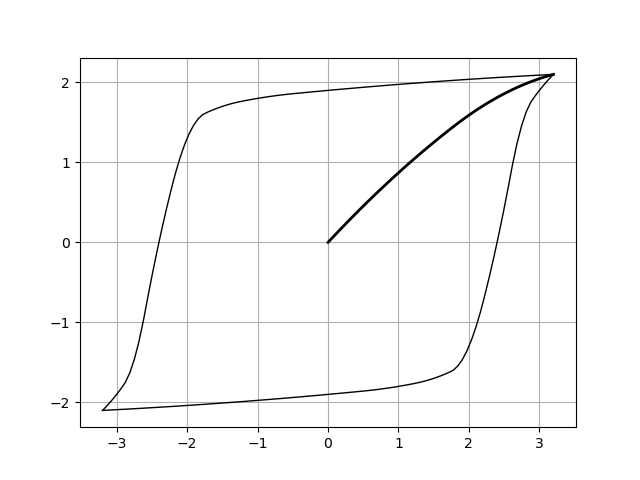
\includegraphics[scale=0.75]{Loop_1}
	\caption{Предельная петля гистерезиса и начальная кривая намагничивания для образца из пермаллоя. Восстановлено по точкам, снятым с экрана ЭО, с помощью кубических сплайнов} \label{Loop_1}
\end{figure}

\begin{figure}[h]
	\centering
	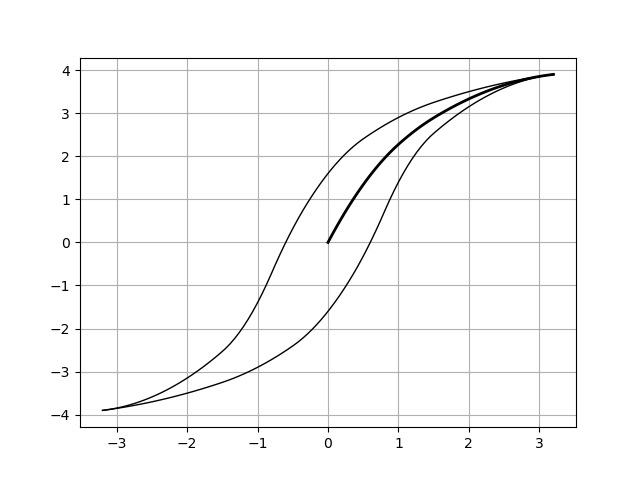
\includegraphics[scale=0.75]{Loop_2}
	\caption{Предельная петля гистерезиса и начальная кривая намагничивания для образца из феррита. Восстановлено по точкам, снятым с экрана ЭО, с помощью кубических сплайнов} \label{Loop_2}
\end{figure}

\begin{figure}[h]
	\centering
	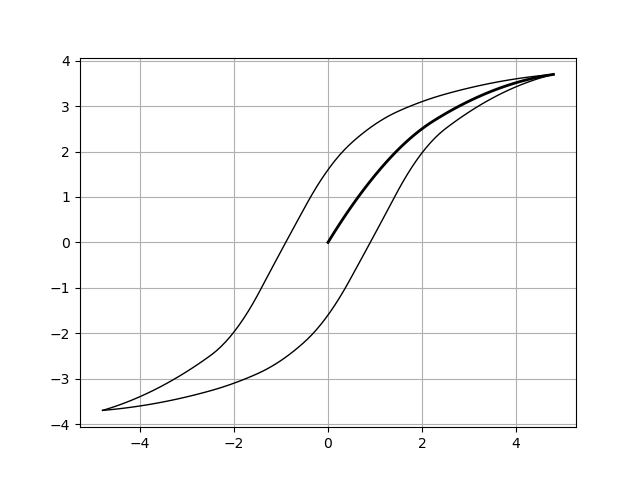
\includegraphics[scale=0.75]{Loop_3}
	\caption{Предельная петля гистерезиса и начальная кривая намагничивания для образца из кремнистого железа. Восстановлено по точкам, снятым с экрана ЭО, с помощью кубических сплайнов} \label{Loop_3}
\end{figure}

\subsection*{II. Проверка калибровки оси $X$ ЭО с помощью амперметра}

Отключим намагничивающую обмотку $N_0$ от цепи, соединив оба провода, идущих к обмотке, на одной из её клемм. С помощью $R_1$ подберём такой ток через сопротивление $R_0$, при котором горизонтальная прямая занимает большую часть экрана ЭО для рабочего коэффицента $K_X=50,0~\frac{\text{мВ}}{\text{дел}}$. Ток через амперметр при этом равен $I_{\text{эф}}=\left(0,583\pm0,004\right)~\text{А}$, сопротивление $R_0=0,3~\Omega$, а горизонтальная прямая на экране занимает $\left(10,0\pm0,1\right)~\text{дел}$ (здесь погрешность определения размер прямой на экране осциллографа равна половине цены малых делений экранной сетки, то есть $0,1~\text{дел}$, а погрешность мультиметра GDM равна $0,005I+15~\text{ед. мл. разряда}$). Тогда чувствительность канала равна $m_X=\left(49,5\pm0,6\right)~\frac{\text{мВ}}{\text{дел}}$, откуда можно заключить, что $m_X=K_X$ в пределах погрешности $\varepsilon_X=1,3~\%$.

\subsection*{III. Проверка калибровки оси $Y$ ЭО с помощью вольтметра}

Соединим вход $Y$ ЭО с клеммами делителя "$\frac{1}{100}$--земля". Не меняя рабочего коэффициента $K_Y=50,0~\frac{\text{мВ}}{\text{дел}}$, подберём с помощью потенциометра $R_2$ напряжение, при котором вертикальная прямая занимает почти весь экран. Подключим вольтметр $V$ к тем же точкам делителя и измерим эффективное значение напряжения. Получим $U_{\text{}}=\left(0,145\pm0,003\right)~\text{В}$ и длину вертикальной прямой $\left(8,0\pm0,1\right)~\text{дел}$, откуда $m_Y=\left(50,4\pm1,0\right)~\frac{\text{мВ}}{\text{дел}}$, откуда можно заключить, что $m_Y=K_Y$ в пределах погрешности $\varepsilon_Y=2,0~\%$.

\subsection*{IV. Определение $\tau$ -- постоянной времени $RC$-цепочки}

Для определения напряжений на входе и выходе интегрирующей ячейки соединим вход ячейки с обмоткой 6,3 В трансформатора. Подключим $Y$-вход ЭО ко входу интегрирующей ячейки и отключим $X$-вход ЭО. Установим чувствительность $K_Y=2,00~\frac{\text{В}}{\text{дел}}$ и подберём с помощью реостата такой ток, при котором вертикальная прямая занимает большую часть экрана, и определим входное напряжение на $RC$-цепочке как $U_{\text{вх}}=2y\cdot K_Y=\left(16,0\pm0,2\right)~\text{В}$.

Теперь, не изменяя тока, переключим $Y$-вход ЭО к выходу ячейки (конденсатору $C$), установим $K_Y=20,0~\frac{\text{мВ}}{\text{дел}}$ и аналогичным образом определим напряжение $U_{\text{вых}}=\left(124,0\pm2,0\right)~\text{мВ}$.

Рассчитаем постоянную времени, получим $\tau=\left(0,408\pm0,008\right)~\text{с}$. Ту же величину через указанные на установке параметры $R_{\text{и}}=20~\text{к$\Omega$}$, $C_{\text{и}}=20~\text{мкФ}$ найдём как $\tau=0,400~\text{с}$. Видим, что полученные значения совпадают в пределах погрешности.

Несложно заметить, что $R=20,0~\text{к$\Omega$}$, $\frac{1}{\Omega C}=159,2~\Omega$, потому условие $R\gg\frac{1}{\Omega C}$ выполняется.

\section*{Вывод}

В данной работе были изучены петли гистерезиса различных ферромагнитных материалов в переменных токах.

В первой части работы были получены предельные петли и начальные кривые намагничивания для образцов из пермаллоя, феррита и кремнистого железа. По точкам, снятым с экрана ЭО, с помощью кубических сплайнов восстановлены петли и кривые (см. рисунки \Ref{Loop_1}, \Ref{Loop_2} и \Ref{Loop_3}). Были рассчитаны цены деления ЭО для петель в $\frac{\text{А}}{\text{м}}$ для оси $X$ и в $\text{Тл}$ для оси $Y$, откуда были найдены коэрцитивная сила $H_c$, индукция насыщения $B_s$ и дифференциальная магнитная проницаемость $\mu_{\text{диф}}$ образцов вблизи нуля (см. таблицу \Ref{Table_1}). Совпадение в пределах погрешности вычисленных значений со справочными  для каждого из образцов говорит о хорошей точности используемого метода и корректности проведения эксперимента.

Во второй и третьей частях работы была проведена проверка калибровок осей ЭО с помощью вольтметра и амперметра. Для рабочих коэффициентов $K_X=50~\frac{\text{мВ}}{\text{дел}}$ и $K_Y=50~\frac{\text{мВ}}{\text{дел}}$ получены значения чувствительности каналов $m_X=\left(49,5\pm0,6\right)~\frac{\text{мВ}}{\text{дел}}$ и $m_Y=\left(50,4\pm1,0\right)~\frac{\text{мВ}}{\text{дел}}$ соответственно, что означает, что в пределах погрешностей чувствительности каналов равны указанным на осциллографе, что ещё раз подтверждает исправность работы ЭО.

В последней части работы  была экспериментально проверена постоянная времени интегрирующей цепочки, которая получилась равной
$\tau=\left(0,408\pm0,008\right)~\text{с}$, т.е. в пределах погрешности совпадающей с $\tau=0,400~\text{с}$, рассчитанной по указанным на установке величинам. Также было подтверждено условие применимости приближений, в которых работает $RC$-цепочка. Полученный результат и его относительно невысокая погрешность подтверждают исправность работы цепочки.

\end{document}
